\documentclass[11pt,chapterprefix=true,pagesize=letter]{scrbook}
\usepackage{etoolbox}
\usepackage[final]{grffile}
\usepackage{graphicx}
\graphicspath{{/home/mkg/images/}}
\makeatletter
\patchcmd{\@@makechapterhead}{.5\baselineskip}{20\p@}{}{}
\makeatother
\usepackage[markuppercase]{scrpage2}
\usepackage{bashful}
\clearscrheadfoot
\ohead{\pagemark}
\ihead{\headmark}
\cfoot[\pagemark]{}
\pagestyle{scrheadings}
\usepackage{lipsum}
\lstdefinestyle{bashfulStdout}{
	basicstyle=\tiny,
	keywords={},
	showstringspaces=false)}

\begin{document}

\title{Selected Photographs}
\author{Michael Gogins \\ \texttt{michael.gogins@gmail.com}}
\maketitle

\chapter*{Introduction}

This book contains my selection of photographs from a lifetime of taking pictures. I have never been a professional photographer, but I was and still am committed to the art of photography. These pictures were variously taken with 35mm film cameras, a variety of digital cameras, and smartphones. They were taken in Utah, the state of Washington, California, New York, other states, and various countries around the world. 

I am a ``street photographer`` with an openness to abstraction. My basic aesthetic is to shoot for what catches my eye and to prize beauty. If I photograph people, I often prefer if they don't know it. My reason for doing photography is to see more truly what God has created.

\chapter*{Photographs}

These images are all in natural color. They are all shot as far as possible without image manipulation. I shoot in JPEG rather than in RAW. Selected metadata from the photographs is used for captioning. If the photograph is a digital scan of a film transparency, the creation date is the date of that scan. The images appear in the order they were taken.


\newpage
\begin{center}
	\includegraphics[width=\textwidth]{c 2013-03-12_12-07-24}
	\bash[stdout]
	exiftool -@ tags '/home/mkg/images/c 2013-03-12_12-07-24.jpg'
	\END
\end{center}

\noindent This is actually a scan of the first photograph I took that I actually liked. It was in 1968 or so in the back yard of my father's girlfriend Doreen's house in Taylorsville, Utah, just after sunset. I believe it was Christmas Day and I had just been given the camera, the entry level Pentax SLR, by my father.


\newpage
\begin{center}
	\includegraphics[width=\textwidth]{c 2013-03-12_12-22-47}
	\bash[stdout]
	exiftool -@ tags '/home/mkg/images/c 2013-03-12_12-22-47.jpg'
	\END
\end{center}

\noindent Ruby Francis, I think in 1977.

\newpage
\begin{center}
	\includegraphics[width=\textwidth]{c 2016-04-06_21-05-56.1}
	\bash[stdout]
	exiftool -@ tags '/home/mkg/images/c 2016-04-06_21-05-56.1.jpg'
	\END
\end{center}

\noindent Deep Creek Mountains, western Utah, 1977 or 1978.

\newpage
\begin{center}
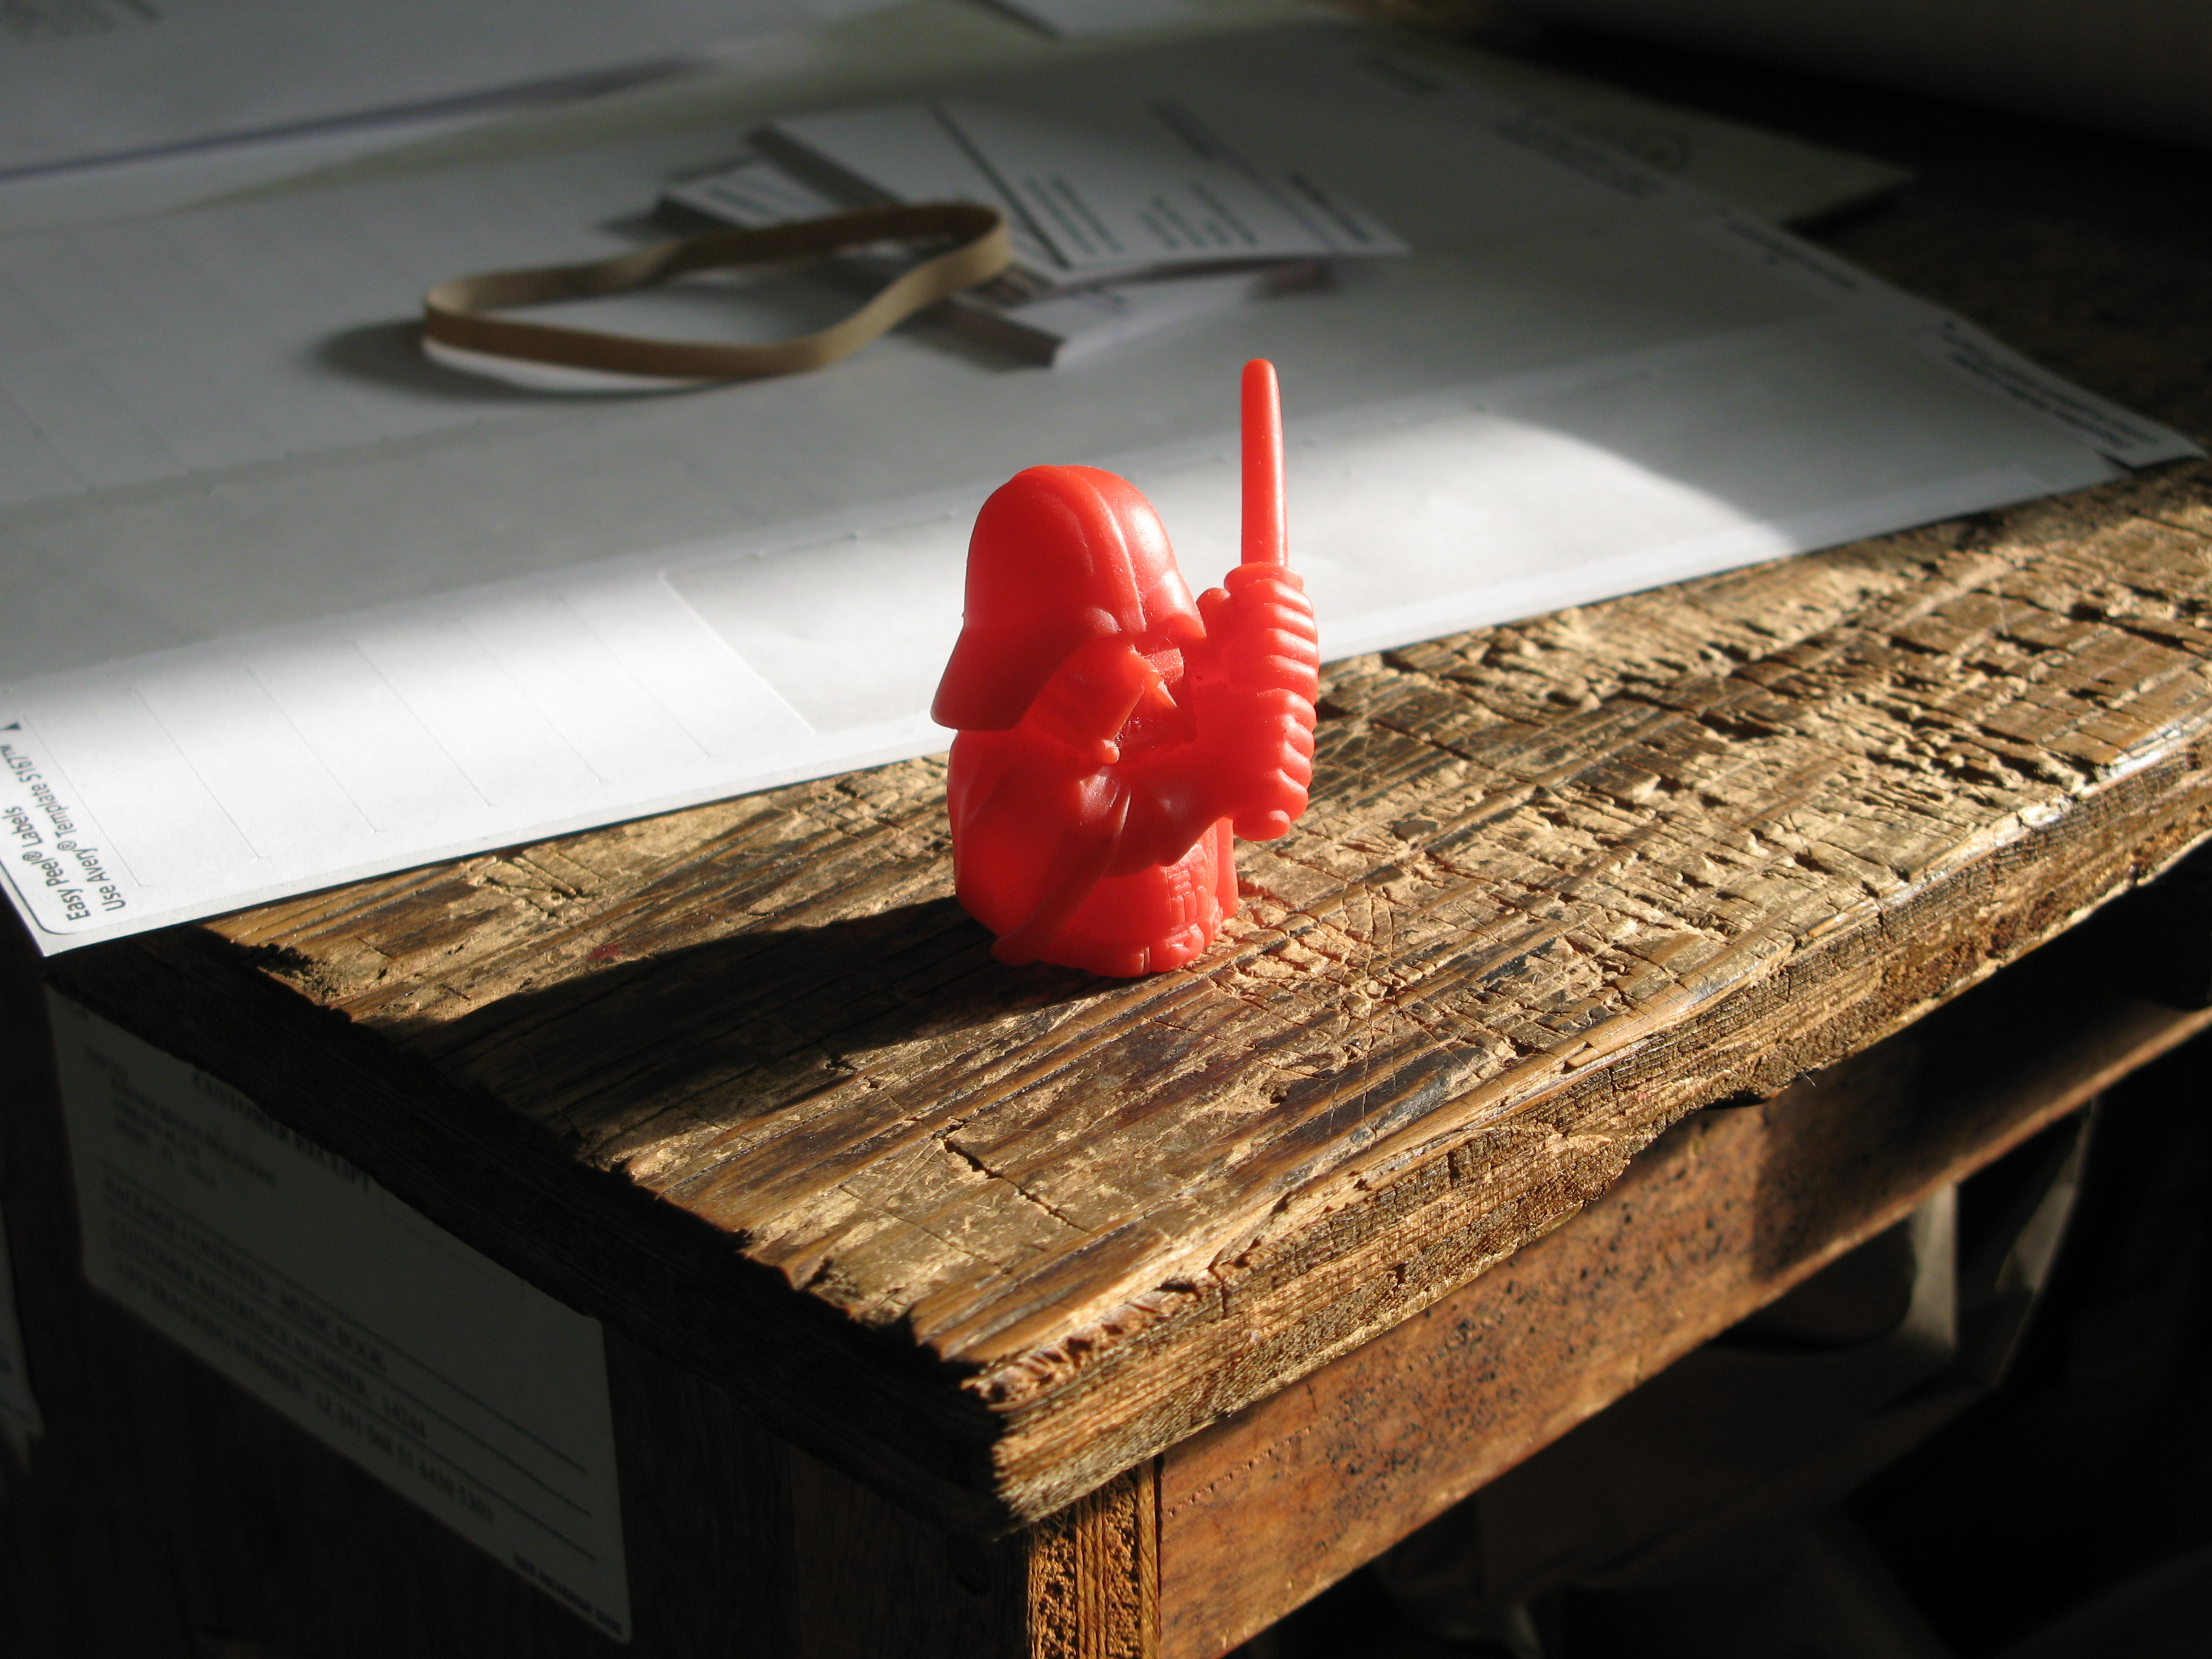
\includegraphics[width=\textwidth]{014.JPG}
\bash[stdout]
exiftool -@ tags 014.JPG
\END
\end{center}

\newpage
\begin{center}
	\includegraphics[width=\textwidth]{"Scan7"}
	\bash[stdout]
	exiftool -@ tags 'Scan7.jpg'
	\END
\end{center}

\newpage
\begin{center}
\includegraphics[width=\textwidth]{"2004-04-13-b 010"}
\bash[stdout]
exiftool -@ tags '2004-04-13-b 010.jpg'
\END
\end{center}

\newpage
\begin{center}
\includegraphics[width=\textwidth]{"2004-12-18a 023"}
\bash[stdout]
exiftool -@ tags '2004-12-18a 023.jpg'
\END
\end{center}

\newpage
\begin{center}
	\includegraphics[width=\textwidth]{"2005-05-17a 042"}
	\bash[stdout]
	exiftool -@ tags '2005-05-17a 042.jpg'
	\END
\end{center}

\newpage
\begin{center}
	\includegraphics[width=\textwidth]{"2009-08-27-a 097"}
	\bash[stdout]
	exiftool -@ tags '2009-08-27-a 097.jpg'
	\END
\end{center}

\newpage
\begin{center}
	\includegraphics[width=\textwidth]{"SM-950U/20180216_201359"}
	\bash[stdout]
	exiftool -@ tags '/home/mkg/images/SM-950U/20180216_201359.jpg'
	\END
\end{center}

\newpage
\begin{center}
	\includegraphics[width=\textwidth]{"SM-950U/20180216_201359"}
	\bash[stdout]
	exiftool -@ tags '/home/mkg/images/SM-950U/20180216_201359.jpg'
	\END
\end{center}


\end{document}
